\documentclass[a4paper,12pt,final]{article}
\usepackage[scaled=0.9]{luximono}
\usepackage[spanish]{babel}
\usepackage[utf8]{inputenc}
\usepackage[T1]{fontenc}
\usepackage{booktabs}
\usepackage{enumitem}
\usepackage{epstopdf}
\usepackage{floatrow}
\usepackage{geometry}
\usepackage{graphicx}
\usepackage{hyperref}
\usepackage{listings}
\usepackage{multicol}
\usepackage{tabularx}
\usepackage{textcomp}
\usepackage{amsmath}
\usepackage{amssymb}
\usepackage{amstext}
\usepackage{caption}
\usepackage{charter}
\usepackage{wrapfig}
\usepackage{amsbsy}
\usepackage{amsthm}
\usepackage{lipsum}
\usepackage{minted}
\usepackage{natbib}
\usepackage{array}
\usepackage{color}
\usepackage{esint}
\usepackage{float}
\usepackage{tikz}

% Tikz Libraries
\usetikzlibrary{positioning}
\usetikzlibrary{arrows}
\usetikzlibrary{shapes}

% Hyperref setup
\hypersetup{
  pdftitle={Procesamiento de datos digitales. Laboratorio 4},
  pdfauthor={Martín Josemaría Vuelta Rojas},
  pdfpagelayout=OneColumn,
  pdfnewwindow=true,
  pdfdisplaydoctitle=true,
  pdfstartview=XYZ,
  plainpages=false,
  unicode=true,
  bookmarksnumbered=true,
  bookmarksopen=true,
  bookmarksopenlevel=3,
  breaklinks=true,
  colorlinks=true,
  linkcolor=blue,
  pdfborder={0 0 0}
}

% Minted settings
\setminted[matlab]{
  autogobble=true,
  linenos=false,
  bgcolor=grey_lighten_4,
  fontfamily=\ttdefault,
  resetmargins=true,
  stripnl=true,
  breaklines=true
  breakautoindent=true,
  breaksymbolleft=\tiny\ensuremath{\hookrightarrow},
  breaksymbolright=\tiny\ensuremath{\hookleftarrow},
  fontsize=\footnotesize
}

\setminted[javascript]{
  autogobble=true,
  linenos=false,
  bgcolor=grey_lighten_4,
  fontfamily=\ttdefault,
  resetmargins=true,
  stripnl=true,
  breaklines=true
  breakautoindent=true,
  breaksymbolleft=\tiny\ensuremath{\hookrightarrow},
  breaksymbolright=\tiny\ensuremath{\hookleftarrow},
  fontsize=\footnotesize
}

\setminted[text]{
  autogobble=true,
  linenos=false,
  bgcolor=grey_lighten_4,
  fontfamily=\ttdefault,
  resetmargins=true,
  stripnl=true,
  breaklines=true
  breakautoindent=true,
  breaksymbolleft=\tiny\ensuremath{\hookrightarrow},
  breaksymbolright=\tiny\ensuremath{\hookleftarrow},
  fontsize=\footnotesize
}

\geometry{
  a4paper,
  total={210mm,297mm},
  left=20mm,
  right=20mm,
  top=20mm,
  bottom=20mm,
}

% \floatsetup[listing]{
%   capposition=top,
%   style=ruled,
% }

% \captionsetup[listing]{
%   labelfont=bf,
%   justification=centering
% }

\floatsetup[figure]{
  capposition=top
}

% \floatsetup[wrapfigure]{
%   capposition=top,
%   style=plain,
% }

\captionsetup[figure]{
  labelfont=bf,
  justification=centering
}

%% LaTeX commands.
\makeatletter
%% -----------------------------------------------------------------------------
% Defining string as labels of certain blocks.
\newcommand{\suma}{\Large$+$}
\newcommand{\inte}{$\displaystyle \int$}
\newcommand{\derv}{\huge$\frac{d}{dt}$}

\definecolor{grey_lighten_4}{rgb}{0.9804, 0.9804, 0.9804}
%% Caption name for minted environments
% \SetupFloatingEnvironment{listing}{name=Script}
% \SetupFloatingEnvironment{listing}{listname=Lista de scripts}
\renewcommand{\listingscaption}{Script}
\renewcommand{\listoflistingscaption}{Lista de scripts}
%% Redefinition of \maketitle command
\def\@maketitle{%
  \newpage%
  \null%
  \vskip 0em%
  \begin{flushleft}%
      \let \footnote \thanks%
      {\LARGE \@title \par}%
  \end{flushleft}%
  \begin{flushright}%
      \vskip 1em%
      {\@author \par}%
  \end{flushright}%
  \noindent\rule{1\columnwidth}{1pt}%
  \par%
}

\makeatother

%% -----------------------------------------------------------------------------
\begin{document}
  \title{\textit{\Large Laboratorio Nº 5}\linebreak{}\linebreak{}
  \textbf{\Huge Filtros}}
  \author{\emph{Martín Josemaría Vuelta Rojas}}
  \maketitle

  \subsection*{Problema 1}
    \noindent Dada la señal en el dominio del tiempo:

      $$x\left(t\right) = \sin\left(t\right) + 0.25\sin\left(10t\right)$$

      \begin{enumerate}[label=\alph*)]
        \item En la gráfica del espectro de potencias, hallar la amplitud,
              la frecuencia y el periodo correspondiente a cada pico.
        \item Diseñe un filtro pasa-bajo y grafique la señal filtrada.
              ¿Cuál es la frecuencia de corte?
        \item Diseñe un filtro pasa-alto y grafique la señal filtrada.
    \end{enumerate}

    \subsubsection*{Solución}

    \noindent La solucion a este problema está contenida en el siguiente \emph{script}
    \begin{listing}[H]
      \label{script:1.1a}
      \inputminted[lastline=21]{matlab}{./laboratorio_5/problema01.m}
    \end{listing}
    \vspace{-1em}
    \noindent {\footnotesize Continúa en la página siguiente\par}
    \vfill

    \newpage
    \noindent {\footnotesize Continuación de la página anterior\par}
    \vspace{-1em}
    \begin{listing}[H]
      \label{scr:1.1b}
      \inputminted[firstline=23,lastline=80]{matlab}{./laboratorio_5/problema01.m}
    \end{listing}
    \vspace{-1em}
    \noindent {\footnotesize Continúa en la página siguiente\par}
    \vfill

    \newpage
    \noindent {\footnotesize Continuación de la página anterior\par}
    \vspace{-1em}
    \begin{listing}[H]
      \label{scr:1.1c}
      \inputminted[firstline=82]{matlab}{./laboratorio_5/problema01.m}
    \end{listing}

    \begin{figure}[H]
      \begin{center}
        \caption{Señal $x\left(t\right)$.}
        \label{p1f1}
        \vspace{-1em}
        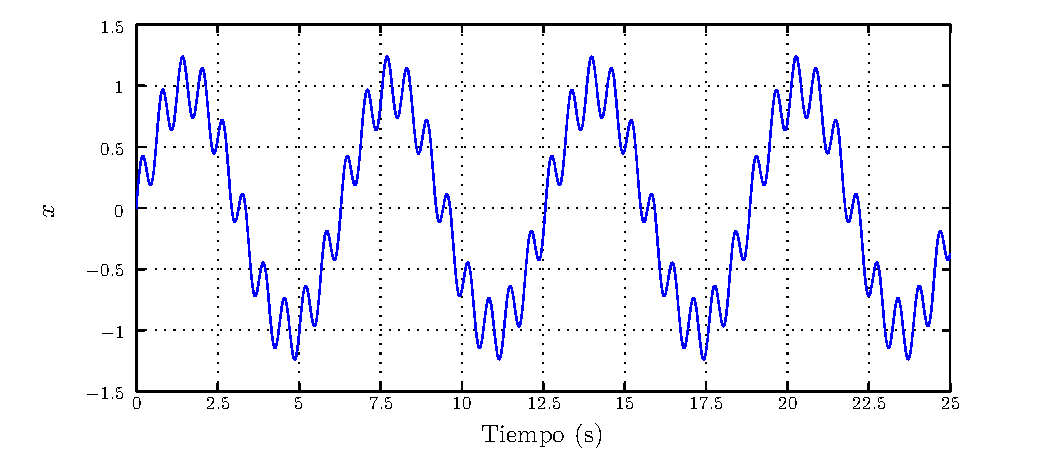
\includegraphics[width=0.9\textwidth]{./laboratorio_5/problema01_signal.pdf}
      \end{center}
    \end{figure}

    \begin{figure}[H]
      \begin{center}
        \caption{Espectro de potencias de la señal $x\left(t\right)$ indiciando los valores de las amplitudes y frecuencias de las componentes la señal..}
        \label{p1f2}
        \vspace{-1em}
        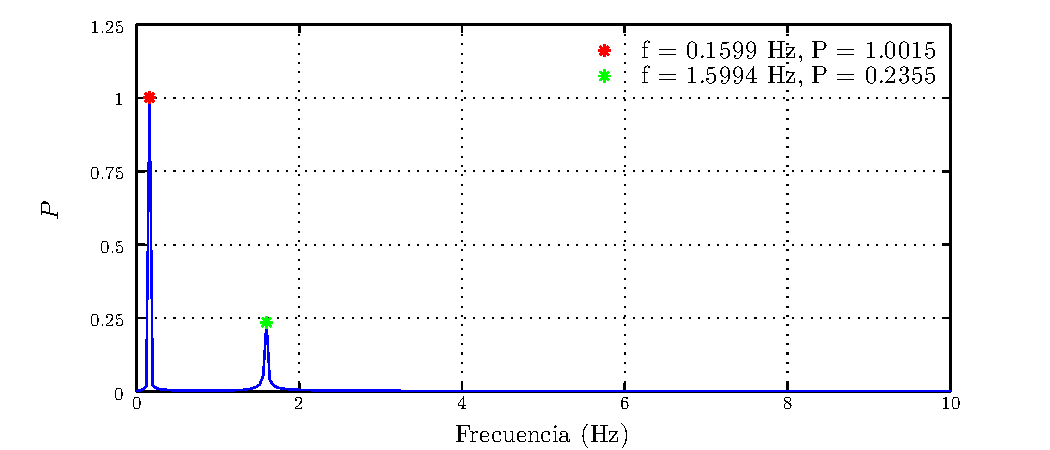
\includegraphics[width=0.9\textwidth]{./laboratorio_5/problema01_power_spectrum.pdf}
      \end{center}
    \end{figure}

    \begin{figure}[H]
      \begin{center}
        \caption{Señal $x\left(t\right)$ sometida a un filtro pasa bajo.}
        \label{p1f3}
        \vspace{-1em}
        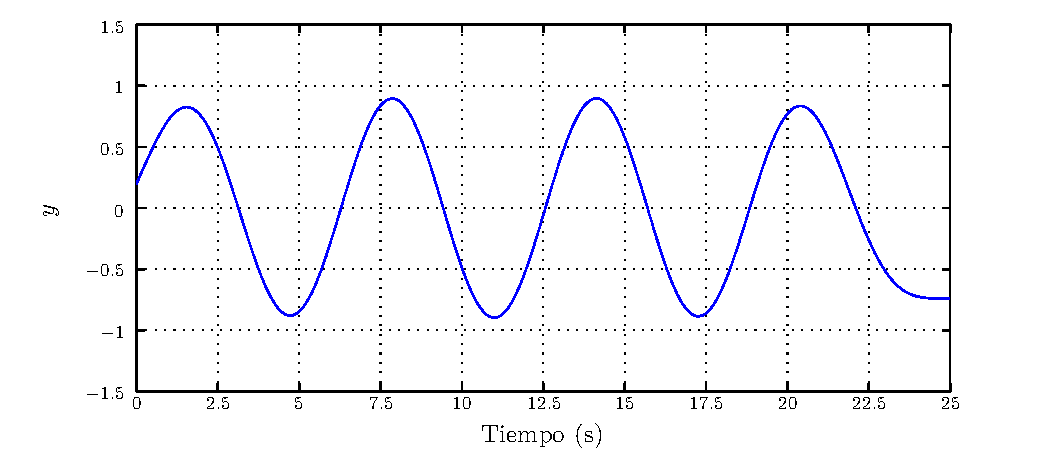
\includegraphics[width=0.9\textwidth]{./laboratorio_5/problema01_lowpass_filtered_signal.pdf}
      \end{center}
    \end{figure}

    \begin{figure}[H]
      \begin{center}
        \caption{Función de transferencia del filtro pasa bajo usado para obtener la fig. \ref{p1f3}. Se muestra la frecuencia de corte del filtro.}
        \label{p1f4}
        \vspace{-1em}
        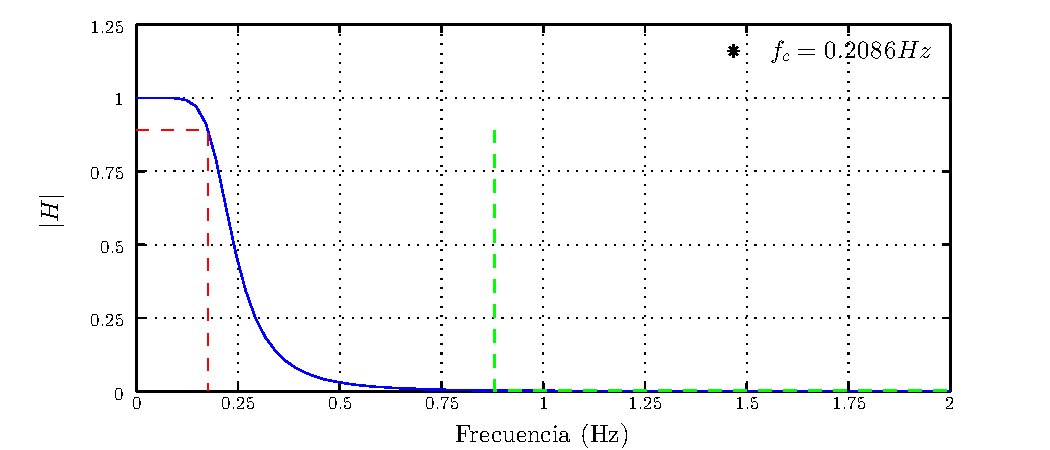
\includegraphics[width=0.9\textwidth]{./laboratorio_5/problema01_lowpass_transfer_function.pdf}
      \end{center}
    \end{figure}

    \begin{figure}[H]
      \begin{center}
        \caption{Respuesta en magnitud del filtro pasa bajo usado para obtener la fig. \ref{p1f3}.}
        \label{p1f5}
        \vspace{-1em}
        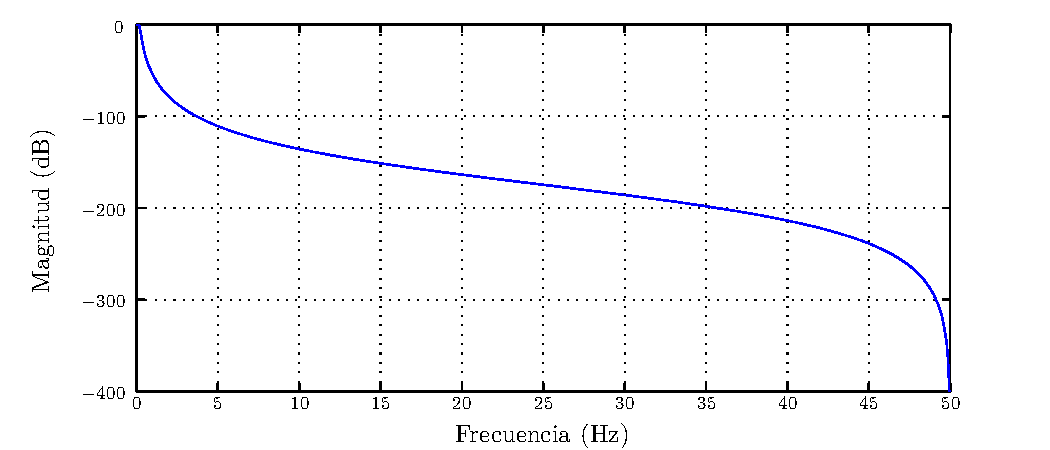
\includegraphics[width=0.9\textwidth]{./laboratorio_5/problema01_lowpass_filter_magnitude.pdf}
      \end{center}
    \end{figure}

    \begin{figure}[H]
      \begin{center}
        \caption{Respuesta en fase del filtro pasa bajo usado para obtener la fig. \ref{p1f3}.}
        \label{p1f6}
        \vspace{-1em}
        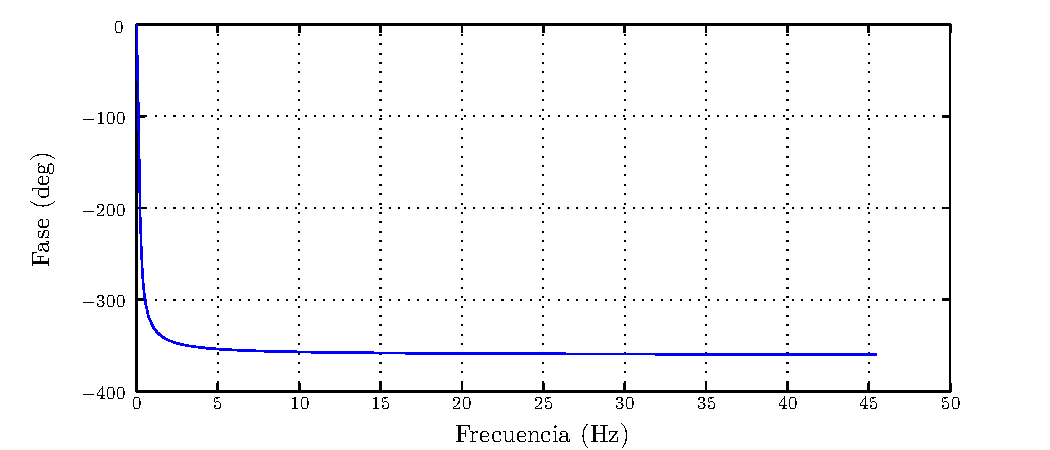
\includegraphics[width=0.9\textwidth]{./laboratorio_5/problema01_lowpass_filter_phase.pdf}
      \end{center}
    \end{figure}

    \begin{figure}[H]
      \begin{center}
        \caption{Señal $x\left(t\right)$ sometida a un filtro pasa alto.}
        \label{p1f7}
        \vspace{-1em}
        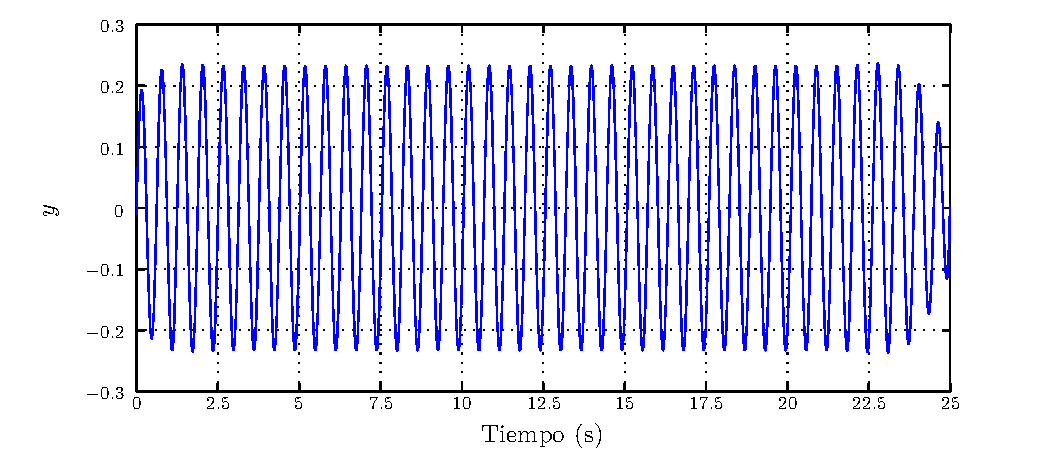
\includegraphics[width=0.9\textwidth]{./laboratorio_5/problema01_highpass_filtered_signal.pdf}
      \end{center}
    \end{figure}

    \begin{figure}[H]
      \begin{center}
        \caption{Función de transferencia del filtro pasa alto usado para obtener la fig. \ref{p1f7}. Se muestra la frecuencia de corte del filtro.}
        \label{p1f8}
        \vspace{-1em}
        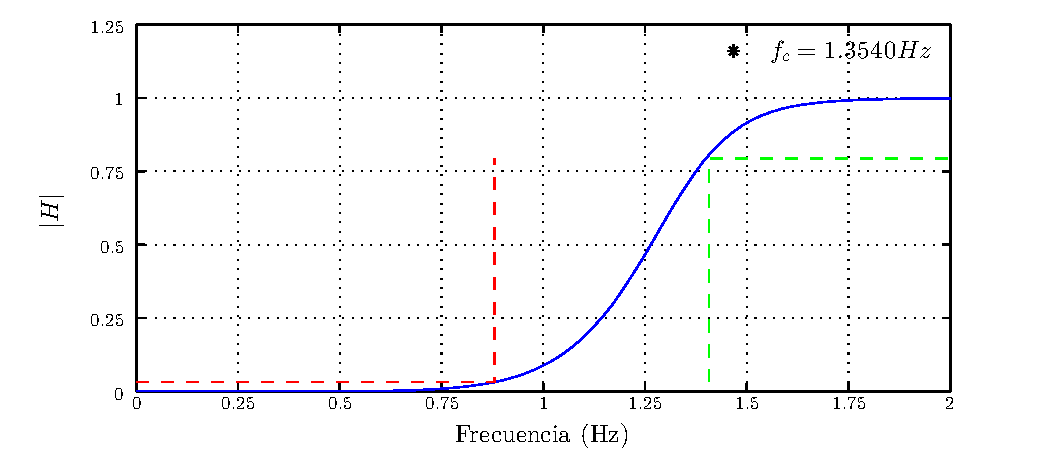
\includegraphics[width=0.9\textwidth]{./laboratorio_5/problema01_highpass_transfer_function.pdf}
      \end{center}
    \end{figure}

    \begin{figure}[H]
      \begin{center}
        \caption{Respuesta en magnitud del filtro pasa alto usado para obtener la fig. \ref{p1f7}.}
        \label{p1f9}
        \vspace{-1em}
        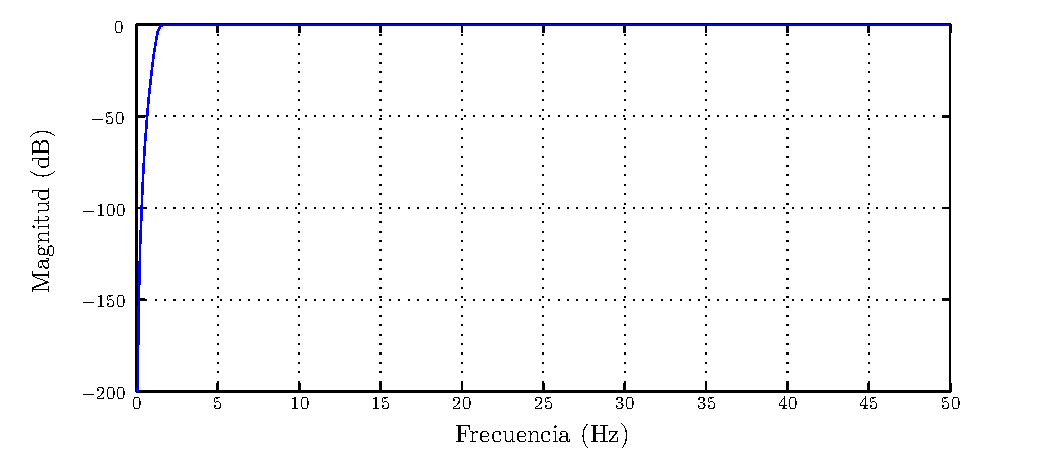
\includegraphics[width=0.9\textwidth]{./laboratorio_5/problema01_highpass_filter_magnitude.pdf}
      \end{center}
    \end{figure}

    \begin{figure}[H]
      \begin{center}
        \caption{Respuesta en fase del filtro pasa alto usado para obtener la fig. \ref{p1f7}.}
        \label{p1f10}
        \vspace{-1em}
        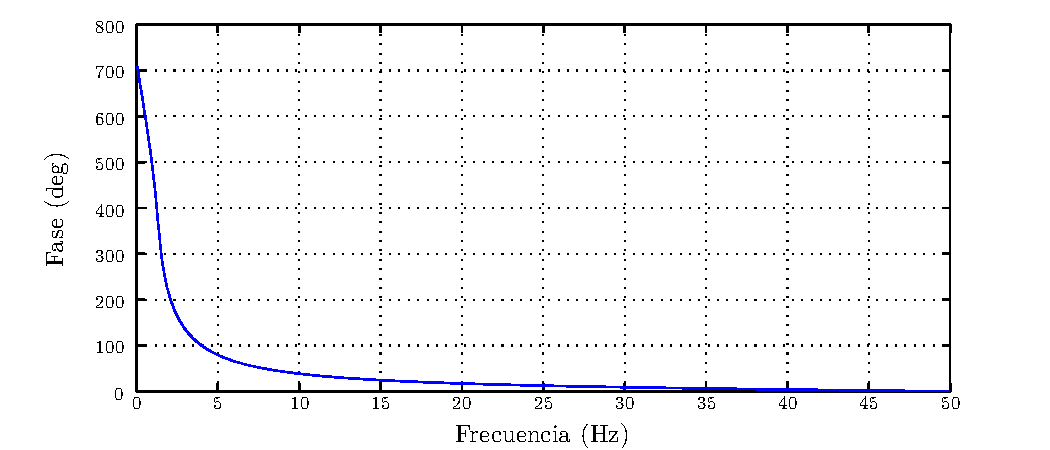
\includegraphics[width=0.9\textwidth]{./laboratorio_5/problema01_highpass_filter_phase.pdf}
      \end{center}
    \end{figure}

  \newpage
  \subsection*{Problema 2}
    \noindent Con el programa de adquisición de datos \texttt{adqsonido.m}, realice
      la grabación durante $5\ s$ de las voces de $2$ personas diferentes.

      \begin{enumerate}[label=\alph*)]
        \item Aplique un filtro pasa-alto con frecuencia de corte de 100 Hz,
              grabe el archivo obtenido.
        \item Calcule la Transformada de Fourier discreta de las dos señales.
              Grafique.
        \item Calcule el coeficiente de correlación entre las TRF de ambas
              señales. ¿Qué puede concluir?
      \end{enumerate}
    \subsubsection*{Solución}

  \newpage
  \subsection*{Problema 3}
    \noindent Descargue el archivo \texttt{pardata.txt}
      \footnote{\url{http://fenlab.9k.com/pds/pardata.zip}} que contiene una
      señal mareográfica real medida en la bahía de Paracas con un sensor
      de nivel ultrasónico

      \begin{enumerate}[label=\alph*)]
        \item Aplique un filtro mediano para eliminar los picos impulsivos. Grafique la señal antes y después de aplicar dicho filtro.
        \item Representar la señal en el dominio de la frecuencia. Identificar los picos principales y periodos de retorno.
        \item Aplicar un filtro adecuado para estudiar las mareas: ¿cuál es el periodo y amplitud de la marea?
        \item Aplicar un filtro adecuado para estudiar las olas: ¿cuál es el periodo y amplitud de las olas?
      \end{enumerate}

      \noindent \emph{Sugerencia}: Revisar el artículo <<Estimación del nivel medio de bajamares de sicigias ordinarias en la bahía de Paracas>>
      \footnote{\url{http://www.rif-fisica.org/images/1/11/111402401.pdf}}.

    \subsubsection*{Solución}

  \newpage
  \subsection*{Problema 4}
    \noindent Se tiene una señal sísmica de tres componentes para la estación de
      Ñaña \footnote{\url{http://fenlab.9k.com/pds/nana.mat}}.

      \noindent La estación está ubicada en :

      \begin{itemize}
        \item Latitud  : $11.988^\circ\ S$
        \item Longitud : $76.842^\circ\ W$
        \item Altitud  : $575\ m.s.n.m$.
      \end{itemize}

      \noindent La ubicación del epicentro fue:

      \begin{itemize}
        \item Latitud    : $15.36^\circ\ S$
        \item Longitud   : $70.90^\circ\ W$
        \item Profundidad: $180\ km$.
      \end{itemize}

      \begin{enumerate}[label=\alph*)]
        \item Graficar la señal para las 3 componentes: Vertical (V), Norte (N), Este (E) en función del tiempo t.
        \item Hallar la distancia epicentral y la diferencia de tiempo de arribo entre la fase P y S.
        \item Hallar el contenido energético promedio de la señal.
        \item Hallar la magnitud del sismo.
      \end{enumerate}

      \noindent \emph{Sugerencia}: Revisar el artículo <<Cálculo de la magnitud sísmica para la estación de Ñaña>>
      \footnote{\url{http://www.rif-fisica.org/images/0/0b/101301755.pdf}}.

    \subsubsection*{Solución}

  \newpage
  \subsection*{Problema 5}
    \noindent Buscar los datos del precio del dólar desde el 1 de enero del 2013
      hasta el 31 de diciembre del 2013.

      \begin{enumerate}[label=\alph*)]
        \item Completar la serie de tiempo para los sábados, domingos y feriados mediante interpolación. Graficar.
        \item Representar la serie en el dominio de la frecuencia. Identificar los picos principales y periodos de retorno.
        \item Filtre las fluctuaciones de alta frecuencia y grafique. ¿Cuál es la tendencia del precio del dólar?
        \item Pronostique el precio del dólar para el 1 de enero del 2014, en base a interpolación polinomial.
      \end{enumerate}

    \subsubsection*{Solución}

\end{document}
